%%%%%%%%%%%%%%%%%%%%%%%%%%%%%%%%%%%%%%%%%%%%%%%%%%%%%%%%%%%%%%%%%%%%%%%%%%%%%%%%
%2345678901234567890123456789012345678901234567890123456789012345678901234567890
%        1         2         3         4         5         6         7         8

\documentclass[letterpaper, 10 pt, conference]{ieeeconf}  % Comment this line out
                                                          % if you need a4paper
%\documentclass[a4paper, 10pt, conference]{ieeeconf}      % Use this line for a4
                                                          % paper

\IEEEoverridecommandlockouts                              % This command is only
                                                          % needed if you want to
                                                          % use the \thanks command
\overrideIEEEmargins


\usepackage[utf8]{inputenc}
\usepackage[T1]{fontenc}

% The following packages can be found on http:\\www.ctan.org
\usepackage{graphics} % for pdf, bitmapped graphics files
\usepackage{epsfig} % for postscript graphics files
%\usepackage{mathptmx} % assumes new font selection scheme installed
%\usepackage{mathptmx} % assumes new font selection scheme installed
%\usepackage{amsmath} % assumes amsmath package installed
%\usepackage{amssymb}  % assumes amsmath package installed

\title{\LARGE \bf
Know Thy Enemy Project
}

\author{Clay Shubert, Lu Liu, Wesley Fortner, and Ethan Ly % <-this % stops a space
}


\begin{document}



\maketitle
\thispagestyle{empty}
\pagestyle{empty}



\begin{abstract}

With the magnitude and frequency of cyber attacks increasing, there is a growing need to be able to identify the point of origins of cyber attacks. For spreading awareness and being prepared for future attacks, it is vital to know as much as possible about the authors of these attacks. KnowThyEnemy is a program that determines the most common origin country of sophisticated attacks (Zero-Day, Ransomware, IoT, etc.) and ranks them according to their effectiveness. By doing so, we hope to bring to light the unknowns about who our enemies are. The information provided here will be helpful to anyone working in the cybersecurity industry who wishes to become familiar with the threats. This data may be utilized by industries in order to better understand their attack surface. 

\end{abstract}



\section{Project Objective}

KnowThyEnemy is a project aims to provide more visibility to industries that are often the targets of sophisticated cyberattacks.
In many cases, industries face a wide variety of attacks, which often requires them to maintain a number of block lists that contain IP addresses and other indicators of previous attempts at an attack. 
There is a potential problem with this because the biggest threat to security is not knowing how it happens, and industries can still be targeted by unique indicators even when they aren't aware of it. 
In order to address this issue, KnowThyEnemy provides a ranking of the most common countries from which sophisticated attacks originate. 
Having this ranking will provide industries with a greater understanding of their attack surfaces, and will enable them to take the necessary precautions in order to protect themselves. 
By utilizing these rankings, industries may choose to geo-block the origin country with the highest ranking if access to this location is not necessary for the operation of their business.
In particular, this may prove useful to small businesses who do not have the resources to keep an ever-changing and extensive block list or the means to pay for such a service from a third party.

\section{Motivation}

The motivation for this project comes from a combination of experience within the cybersecurity field and an interest in becoming involved. 
The connection between threat actors and their location is an interesting topic and we are interested in investigating whether there is a correlation between the location of attack and the sophistication of the attack. 
Additionally, we are interested in exploring how open-source can be used to analyze and visualize data to provide solutions to real-world problems. For the purpose of future threat awareness, learning how to use these open source tools will be extremely valuable. In the future, we will be able to apply these skills directly to a wide range of opportunities in industries as well as in the workforce as a whole.

\section{Data Sources}

The data sources for this project will be the following:

\begin{itemize}
    \item \textbf{AlienVault OTX:} AlienVault Open Threat Exchange (OTX) is an open information-sharing and analysis network that provides real-time, actionable threat intelligence. AlienVault OTX provides an API that allows users to retrieve this data programmatically. 
    \item \textbf{VirusTotal:} VirusTotal is a free service that analyzes suspicious files and URLs and facilitates the quick detection of viruses, worms, trojans, and all kinds of malware. It is a repository of known malware samples and a service that analyzes them. VirusTotal provides an API that allows users to retrieve this data programmatically.
    \item \textbf{AbuseIPDB:} AbuseIPDB is a free project to check IP address reputation. It includes information about the IP such as Country Name, Hostname, Email, Community Rating, etc. The project is used by tens of thousands of users every day. AbuseIPDB provides an API that allows users to retrieve this data programmatically.
    \item \textbf{URLhaus:} URLhaus is a project by abuse.ch that is aimed at providing a respository of malicious URLs that are being used by malware distribution groups for the purpose of sharing malicious URLs. This service is community based, allowing users to upload and help protect other users out there. URLhaus provides an API that allows for the retrieval of this data programmatically many different formats.
\end{itemize}

\section{Member Responsibilities}

\begin{itemize}
    \item \textbf{Clay Shubert:} Clay was responsible for the data collection and analysis of all AlienVault OTX collection process. Clay also contributed to the creation and writing of the Project Proposal report, final project report, and final project presentation.
    \item \textbf{Lu Liu:} Lu was responsible for the data collection and analysis of URLHaus, as well as visualization of URLHaus data. As part of her work, she also contributed to the preparation of the final report and presentation for the project.
    \item \textbf{Wesley Fortner:} Wesley was responsible for the data collection and analysis of AlienVault OTX Data. Wesley also was responsible for the project report and presentation creation.
    \item \textbf{Ethan Ly:} Ethan will be responsible for the data collection and analysis. He primarily worked on the URLHaus approach for data collection. However, Ethan assisted Clay and Wesley with AlienVault OTX data analysis as well. Ethan also worked on the project final report and helped to create and present the final project presentation.
\end{itemize}

\section{Models or Algorithms Used}

    \subsection*{OTXv2}
    OTXv2 is a Python library serves as an interface for interacting with the AlienVault OTX API. In our project, we utilized this model to extract data from the AlienVault OTX API. By employing a complimentary API key, we successfully retrieved approximately 6,000 posts and in excess of 35,700 IPv4 addresses. These resources were subsequently geo-located and analyzed over a recent 90-day period.

    \subsection*{Pygal}
    Pygal is an open-source Python library that allows users to create easy-to-read visual and interactive graphs/charts in SVG format. In our study, we employed Pygal to enhance the visualization of data derived from pinpointing the geographic locations of IP addresses. 
    The data we gathered was effectively projected onto a world map. This map highlights the top 10 countries identified as primary sources of specific attacks, with each country being distinctly color-coded for enhanced readability.
    
    \subsection*{IPLocation API}
    IPLocation, a complimentary API, offers the functionality of returning the country of origin for submitted IP addresses. While this API initially appeared promising, our research objectives required an API providing more detailed geographic location data, including country, region, and city. 
    Although APILocation does offer this extended data set, encompassing ISP, organization, latitude, and longitude, these features are accessible only through a paid subscription. Consequently, our team decided to explore alternative URL APIs. 
    Despite many of these alternatives imposing limitations on the number of permissible calls within a specific time frame, they were deemed capable of furnishing the comprehensive data required for our study.
    
    \subsection*{URLHaus}
    URLHaus operates as a community-driven service aimed at establishing a database where users can share information about malicious URLs. This database includes details such as the URL's current status (online or offline) and various associated tags (e.g., 32-bit download, elf, mozi). The service offers an API equipped with a range of functionalities, including the submission of URLs and the export of collected payloads. However, for our research purposes, we primarily utilized the API for its database dump feature, available in CSV format. This format was particularly conducive to our Python script, enabling the extraction of each URL for subsequent submission to the URLScan API, as detailed in the following section. Given the nature of the data, comprising numerous URLs with malicious intent, it was imperative to exercise heightened caution during the handling process.
    
    \subsection*{URLScan}
    URLScan, a complimentary service, provides the capability to scan website URLs and analyze an array of associated metadata. In our project, we utilized its free API, but encountered limitations in the API's usage capacity. As previously mentioned, URLHaus offers an export feature for a comma-separated value (CSV) file, containing a list of malicious URLs from a specified timeframe. We integrated this CSV file into a Python script, which was then used to make API calls to URLScan, enabling us to retrieve the desired metadata.

    The data extracted from these API calls was extensive, including details such as the time of scan, the URL, and server information. Although the API returned close to 40 different data fields, our primary focus was on extracting the IP address and geographical location data, particularly the country and city. This targeted approach allowed us to concentrate on the most relevant data for our analysis. 
    
    \subsection*{Python}
    All data collection and analysis was done using the programming language of Python. 

\section{Results}
\begin {table}[h]
\small
\begin{tabular}{ || p{6em} | p{4.2cm}| p{1cm} | p{2cm} | p{1cm} || } 
\hline
 Country & Number of recorded IPs Associated with attack\\ 
 \hline\hline
 1. China & 1750\\ 
 \hline
 2. United States & 1192\\
 \hline
 3. Brazil & 723\\
 \hline
 4. India & 626\\
 \hline
 5. Russia & 540\\
 \hline
 6. Korea & 424\\
 \hline
 7. Vietnam & 393\\
 \hline
 8. Indonesia & 197\\
 \hline
 9. Venezuela & 197\\
 \hline
 10. Taiwan & 183\\
 \hline
\end{tabular}
\end {table}
After gathering data, we were able to visually compile all the data and analyze it. We collected 606 reports of cyber attacks from the open source AlienVault OTX platform. From these 606 reports, we were able to over 9,000 IP addresses that were associated with the attack. Once we had this large data source of IP addresses we were able to visualize our data by country of origin. The map of our final data can be viewed below as figure 1.  
We saw China come in first place on the list, shortly followed by the United States. To somewhat of a surprise, we saw Brazil come in at third place, followed by India at fourth place, and Russia at fifth place. We somewhat hypothesized that the list would loosely correlate to the most populous countries in the world. We decided to include that list in this report so we could compare and contrast the changes between the lists.
\begin{figure}[h]
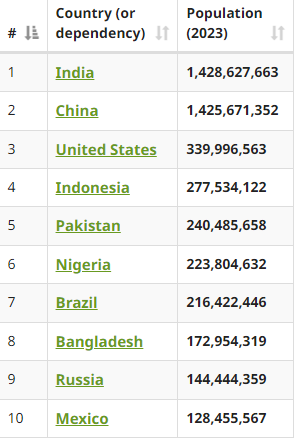
\includegraphics[width=8cm,height=10cm]{figures/top10population.png}
\caption{Top 10 World Populations}
\end{figure}
Given the population size of China and it's well known and established technology dependent society, we expected to see China near the top of the list. Also, we expected to see United States atop the list because of the ease of accessibility of any forms of technology which is similar to that of China. We were definitely somewhat surprised to see Brazil in the third position because Brazil typically is not in the spotlight when it comes to talks surrounding cyber threats like China and the United States are. Another interesting thing we saw from the results was that there were no Western European countries in the list. We would have expected to at least see one highly populated Western European country make it on the final list but they surprisingly did not.
\begin{figure*}[h]
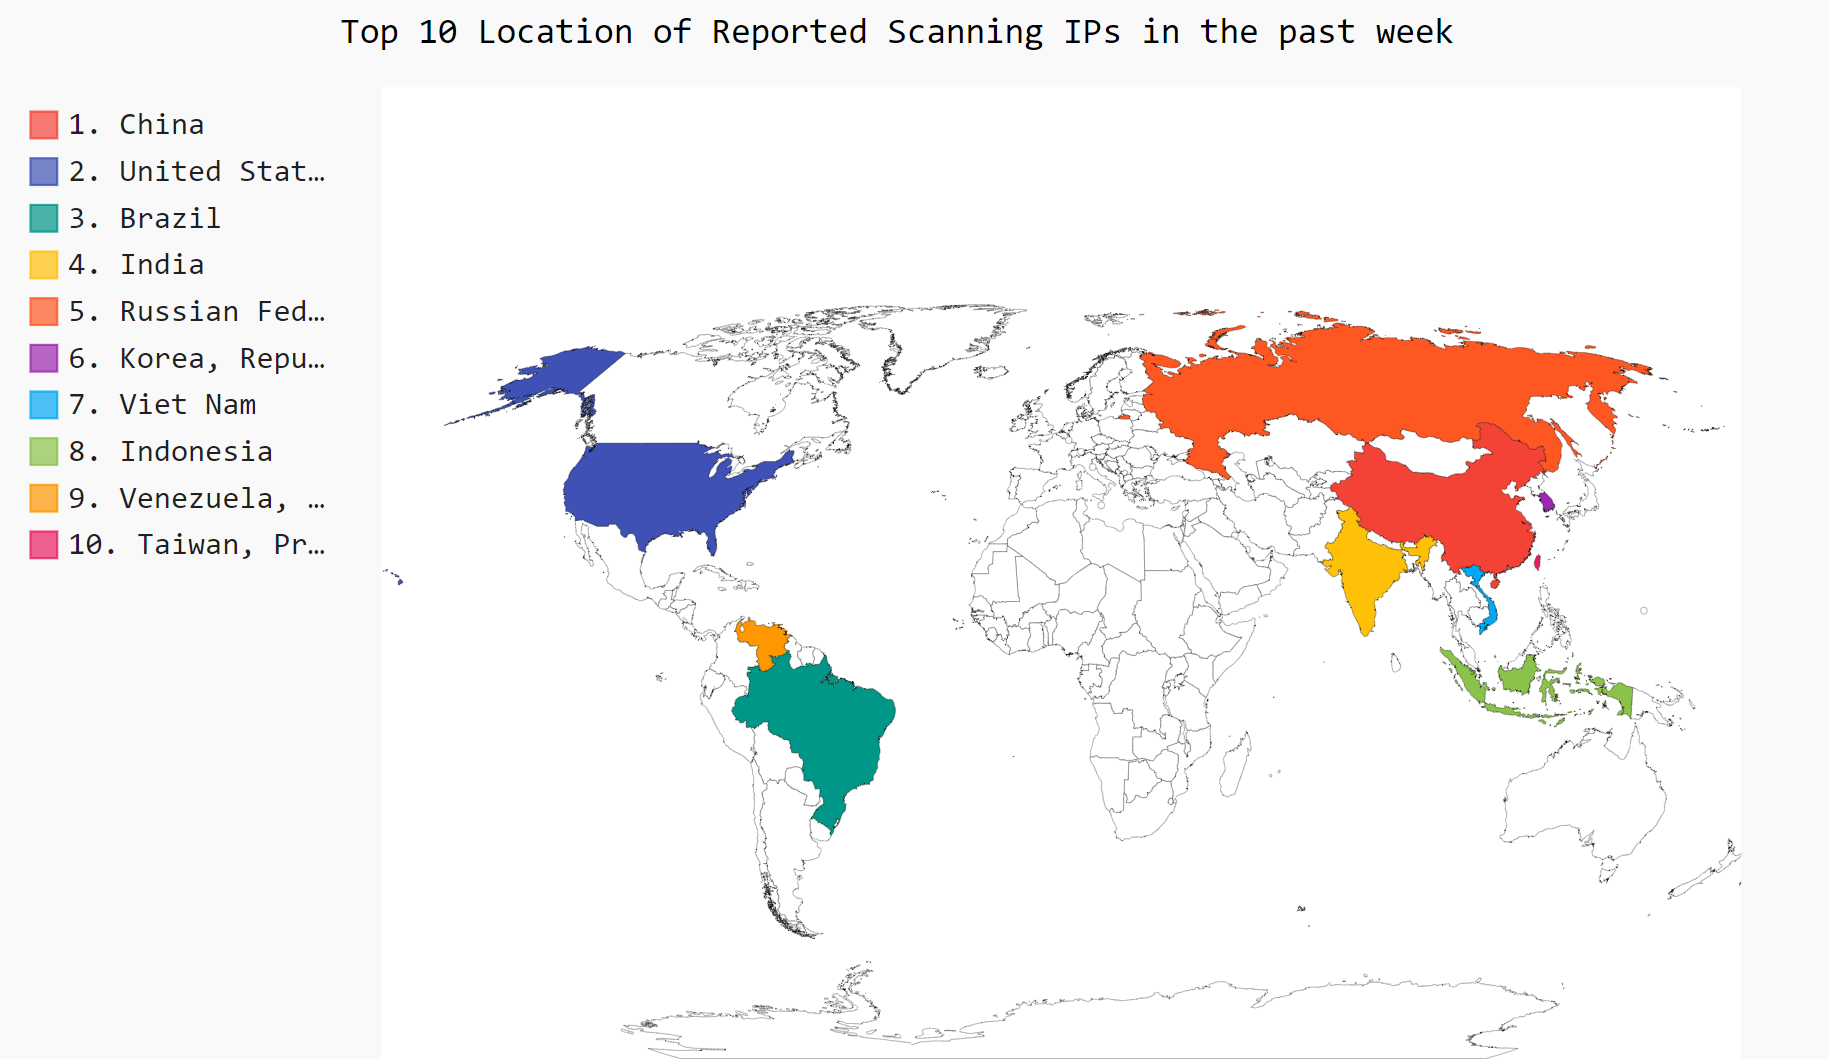
\includegraphics[width=\textwidth,height=10cm]{figures/top10pic.png}
\caption{Cyberattacks by Country}
\end{figure*}
\section{Primary Issues Encountered}
\subsection*{AlienVault OTX Issues}
Due to the setup of AlienVault OTX and how their API is configured, we were somewhat limited in the amount of data we could collect. We were also limited by the length of the semester and the time frame this project sat in. We were collecting data from AlienVault OTX in real time which put a constraint on us because the data we could collect was within the boundaries of the semester. Ideally, we would have liked to continually collect data across an entire year. Also, we ran into more issues with the amount of data that we could collect with the API. Without paying for a higher level of license with AlienVault OTX, we had a monthly limit of data usage with the AlienVault OTX OTXV2 API. We had to tread carefully knowing we had a usage limit. This issue limited the amount of experimentation we could do with API in our research phase. 
\subsection*{URL Scanning}
As mentioned previously, there were various options for URL scanning that we used. Each provided different information regarding the URL but most provided what we needed (geographic location). URLs with malicious content were publicly posted on URLHaus which allowed for a database dump that could be fed into the URL scanning APIs. This is where some problems were encountered. When scanning these URLs and retrieving only certain data from the JSON, it required a ton of string extraction, removal, and concatenation. It seemed unnecessary to store all of the data returned by the URL scan so this was a necessary step to be able to only store geographic location data such as country, city, and region of the attack. Just as AlienVault OTX had API call limits, our URL scanning APIs also had this. Due to the vast amount of malicious URLs dumped into the CSV file, it became clear that the API calls would reach the limit fairly quickly. This made it hard to develop for long periods of time due to running out of calls simply while testing. Finally, the last issue ran into while attempting to scan these URLs was in relation to the constant updating of these malicious links listed on the URLHaus database. Each posted URL can either be active or inactive. Therefore, if a URL is inactive, the scan will not return valid data and the URLHaus database is only as up-to-date as the users make it to be. This means that even URLs with an "active" tag may possibly be inactive and vice versa. This made collecting valid data somewhat difficult as again, we had limited API calls.

\section{Future Work}
\subsection*{Expanded Data Collection Window}
In considering future research directions, it becomes evident that there exists a substantial, yet largely unexplored, research domain related to our current work, particularly given the limited duration of data collection in this project. Our engagement with AlienVault OTX was constrained to a specific timeframe, aligning with the academic semester, which inevitably restricted the scope of our data gathering. However, we recognize the potential benefits of extending our data collection over longer periods.

Such an extended timeframe would enable us to uncover diverse avenues and trends within the collected data. For instance, a more prolonged data collection phase would allow for a detailed analysis of geo-located data trends and their correlation with seasonal changes throughout the year. Additionally, it would offer an opportunity to examine how these geo-location trends interact with contemporary events, socio-economic developments, and other significant real-world occurrences. This approach would not only broaden the scope of our research but also enhance our understanding of the intricate relationship between digital data trends and global events.

\subsection*{World Event Correlations}
This project holds the potential to be particularly insightful during major global conflicts. An area of compelling interest would be to delve deeper into world events, such as the conflict between Russia and Ukraine. Analyzing cyber-attacks emanating from these specific regions could reveal patterns in the escalation or de-escalation of such activities, correlating with the evolving relations between the countries involved.
However, the complexity and scope of such an analysis extend beyond the confines of a single semester project. It necessitates precise timing in data collection and the ability to maintain an extended period of data gathering. This approach would ensure a comprehensive understanding of the cyber dynamics in the context of global geopolitical events, providing valuable insights into the intersection of international relations and cyber activities.

\subsection*{Analysis of Specific Types of Attacks}
The temporal constraints of the academic semester significantly limited the depth of exploration possible within this project. For future research, it would be meaningful to investigate specific types of cyber-attacks and examine potential correlations between the nature of these threats and their respective countries of origin. Such an investigation could reveal whether certain countries are more prone to employing specific methods of cyber-attack. This line of inquiry promises to be an intriguing avenue, potentially uncovering patterns of cyber activity unique to particular regions and contributing to a more nuanced understanding of global cyber threat landscapes.

\section{Milestones and Organization Chart}

    \subsection*{Milestone 1: Data Collection}
    \begin{itemize}
        \item \textbf{Description:} Collect data from the data sources listed above.
        \item \textbf{Due Date:} 10/15/2023
        \item \textbf{Responsible Members:} All
    \end{itemize}
    \subsection*{Milestone 2: Data Analysis}
    \begin{itemize}
        \item \textbf{Description:} Analyze the data collected and determine the most common origin countries of sophisticated attacks.
        \item \textbf{Due Date:} 10/31/2023
        \item \textbf{Responsible Members:} All
    \end{itemize}
    \subsection*{Milestone 3: Data Visualization and Error Correction}
    \begin{itemize}
        \item \textbf{Description:} Visualize the data and correct any errors.
        \item \textbf{Due Date:} 11/15/2023
        \item \textbf{Responsible Members:} All

    \end{itemize}
    \subsection*{Milestone 4: Project Presentation}
    \begin{itemize}
        \item \textbf{Description:} Create the project presentation.
        \item \textbf{Due Date:} 12/05/2023
        \item \textbf{Responsible Members:} All
        \item \textbf{Deliverable:} Project Presentation
    \end{itemize}
    \subsection*{Milestone 5: Project Report}
    \begin{itemize}
        \item \textbf{Description:} Write the project report.
        \item \textbf{Due Date:} 12/12/2023
        \item \textbf{Responsible Members:} All
        \item \textbf{Deliverable:} Project Report
    \end{itemize}

    


\section{Conclusion}

At the end of the project, we provided deliverables that included a project report and presentation outlining the details of our work. 
In addition, we delivered that presentation to the class outlining our findings and results. Lastly, we built a working program that can be used to determine the most common origin countries of sophisticated attacks. After reflecting on our results and findings, we believe that this was a really beneficial project that brought some interesting findings into the light. We discovered that one of the largest sources of threats originate from our own country. We also discovered the current sources of other major threats and threat actors which consisted of countries like China, Brazil, Russia, and India. We analyzed this data and look for correlations relating to world populations. We were limited in the amount of data we could collect at times; however, we feel were able to compile some meaningful and insightful results. We hope that this project is helpful to anyone who is interested in seeing current threats and determining the locations of their enemies.   


\begin{thebibliography}{1}

\bibitem{b1}
Abuse.ch, ``URLhaus Browse'' [Online]. Available: \href{https://urlhaus.abuse.ch/browse/}{} [Accessed: Dec. 11, 2023].
\bibitem{b2}
AlienVault, ``Browse Global Pulses,'' [Online]. Available: \href{https://otx.alienvault.com/browse/global/pulses}{}
[Accessed: Dec. 11, 2023].

\end{thebibliography}



\end{document}
